\section{Evaluation}

\subsection{Text size importance in stylometry}

Figure~\ref{img:degradation} shows the importance of having texts large enough for a correct stylistic detection using distance between MFW vectors.

PAN16 dataset is a difficult dataset due to its small size, thus extracting reliable feature for each text to estimate each style is also a difficult task.
After multiple tests, the PAN @ CLEF 2016 dataset was not used further in this study due to its difficulty in finding reliable stylographic clues.

\begin{figure}
  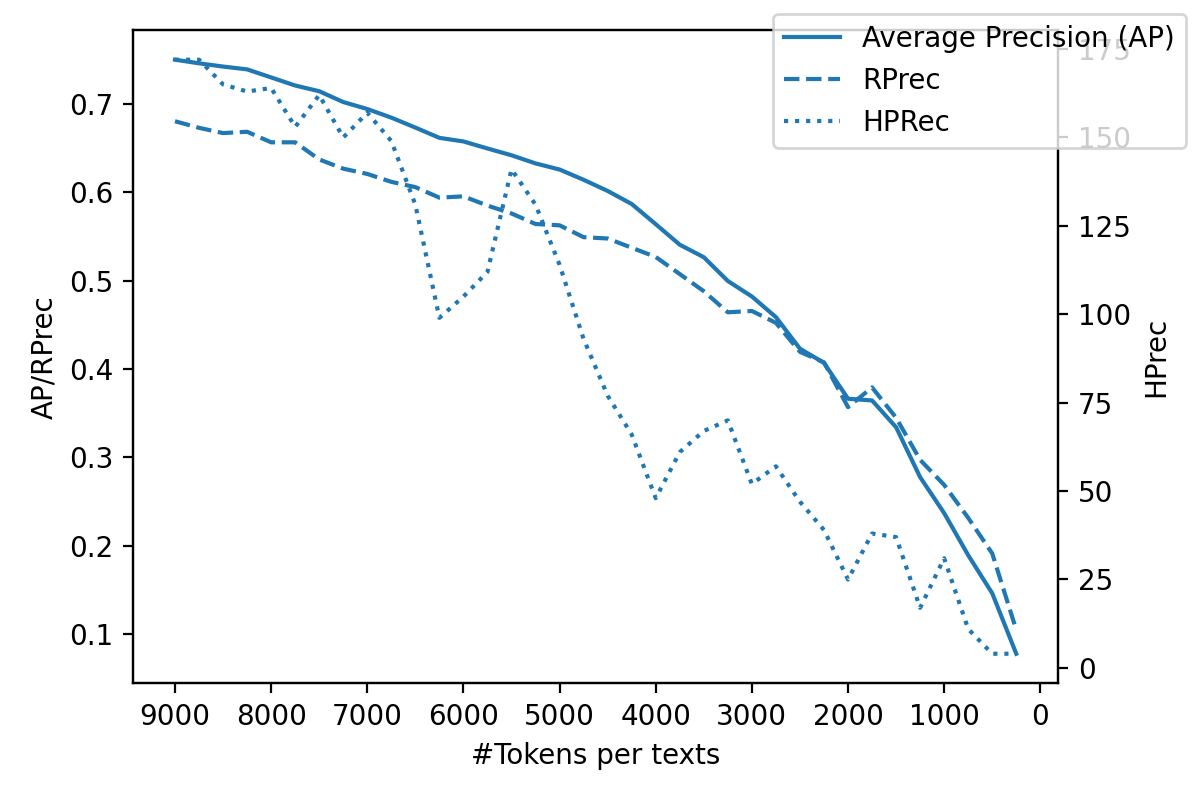
\includegraphics[width=\linewidth]{img/degradation.png}
  \caption{St-Jean ranks list evaluation on AP, RPrec and HPrec over the text size. Rank list computed using 500 MFW and the zscored-normalized cosine distance}
  \label{img:degradation}
\end{figure}


\subsection{Rank list evaluation}

Some of the definitions in this sections are an adapted version of the ones in~\cite{kocher_linking},~\cite{bcubed}.

\begin{definition}[Relevant link~\cite{kocher_linking}]
  A relevant link is a link in the relevant set.
  \begin{equation}
    relevant(l_i) =
    \begin{cases}
      1, & if\ l_i \in R \\
      0, & otherwise
    \end{cases}
  \end{equation}
\end{definition}

\begin{definition}[Precision@k~\cite{kocher_linking}]
  The precision@k is a function which take a integer k, with k < |L|
  \begin{equation}
    precision(k) = \frac{1}{k} \sum_{j=1}^{k} relevant(j)
  \end{equation}
\end{definition}

\begin{definition}[Average Precision (AP)]
  The mean over the precision@k each time a relevant link is retrieved.
  \begin{equation}
    AveragePrecision = \frac{1}{|R|} \sum_{j=1}^{|L|} precision(j) \cdot relevant(j)
  \end{equation}
\end{definition}

\begin{definition}[RPrec~\cite{kocher_linking}]
  The RPrec is the precision in the rank list at rank |R|.
  With R being the relevant set. (Not to be confused with the r ratio)
  \begin{equation}
    RPrec = precision(|R|)
  \end{equation}
\end{definition}

\begin{definition}[HPrec~\cite{kocher_linking}]
  The HPrec represent a maximal rank j in the rank list where the precision is still 100\%.
  This value is in the range [0 - |R|].
  0 means the first pair in the rank list is incorrect.
  |R| means every true links are ranked in the top part of the rank list.
  \begin{equation}
    HPrec = \max\{i \in \mathbf{N} | precision(i) = 1\}
  \end{equation}
\end{definition}


\subsection{POS n-grams}

Figure~\ref{fig:pos_ngrams} show the average precision on the rank list produced by using POS n-grams over the number of MFW (most frequent word, in this case POS n-grams are considered as words).
The two following informations can be intuitively observed on this plot:

A more complex POS n-gram requirement more MFW to archive its maximal effectiveness.
In the St-Jean corpus 26 POS are used to describe every words in the corpus.
Which correspond to $26^2 = 676$ possible unique POS 2-grams, to $26^3 = 17'576$ POS 3-grams and $26^4 = 456'976$.

Like the other methods, an overfit to less important words is possible if the MFW ceiling is too high, reducing the average precision.
In Figure~\ref{fig:pos_ngrams} the POS 2-grams clearly have drop in average precision after \~250-MFW.

\begin{figure}
  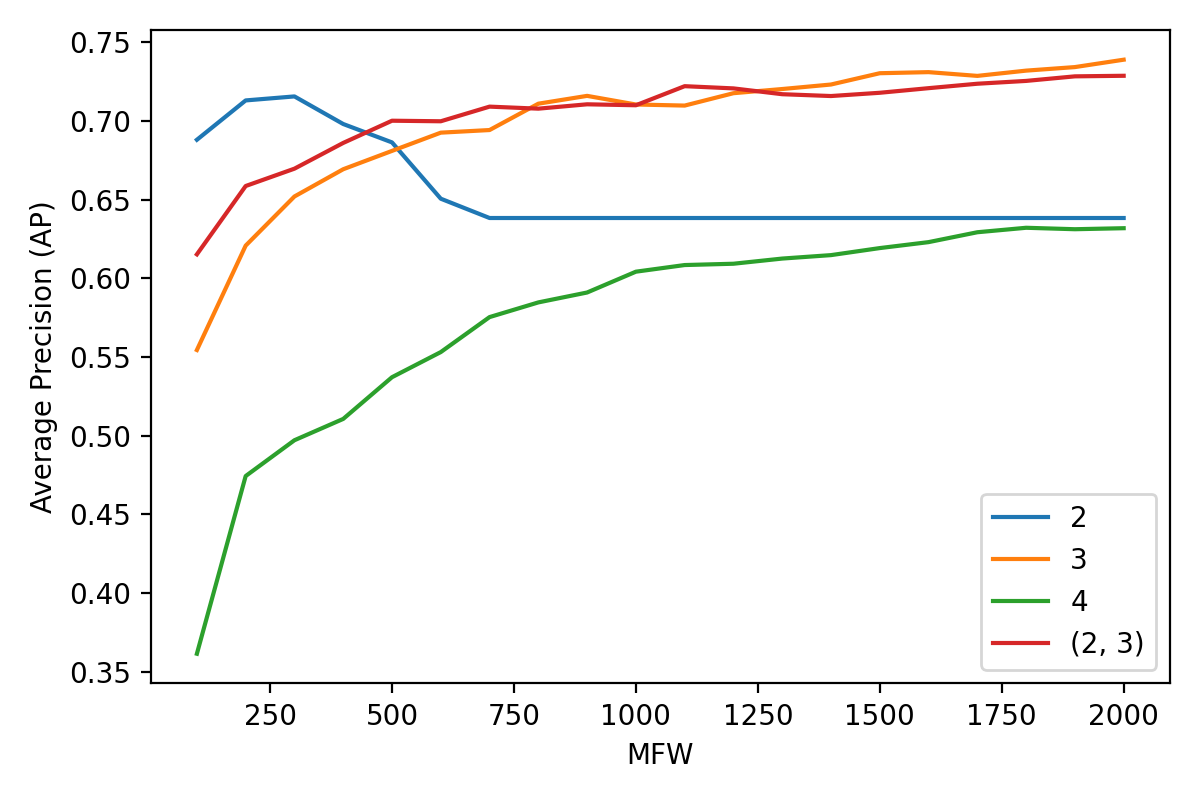
\includegraphics[width=\linewidth]{img/pos_ngrams.png}
  \caption{Average precision over the MFW in the rank list generated using the z-score normalized cosine distance.}
  \label{fig:pos_ngrams}
\end{figure}

\subsection{First letters, last letters of tokens}

With this methods, the goal is to extract the N first letter of each word tokens which correspond generaly to the meaning of a word.
This approach is closely related to the lemma approach.
Extract also the N last letter of each word tokens which in this case correspond to the role of the word in a sentence.
This second approach is closely related to the POS approach.
These two methods can be considered as a simplified n-grams approach.

Figure~\ref{fig:first_last_letters_ngrams} shows the average precision using the z-normalized cosine distance on the experiment for N = 4.

\begin{figure}
  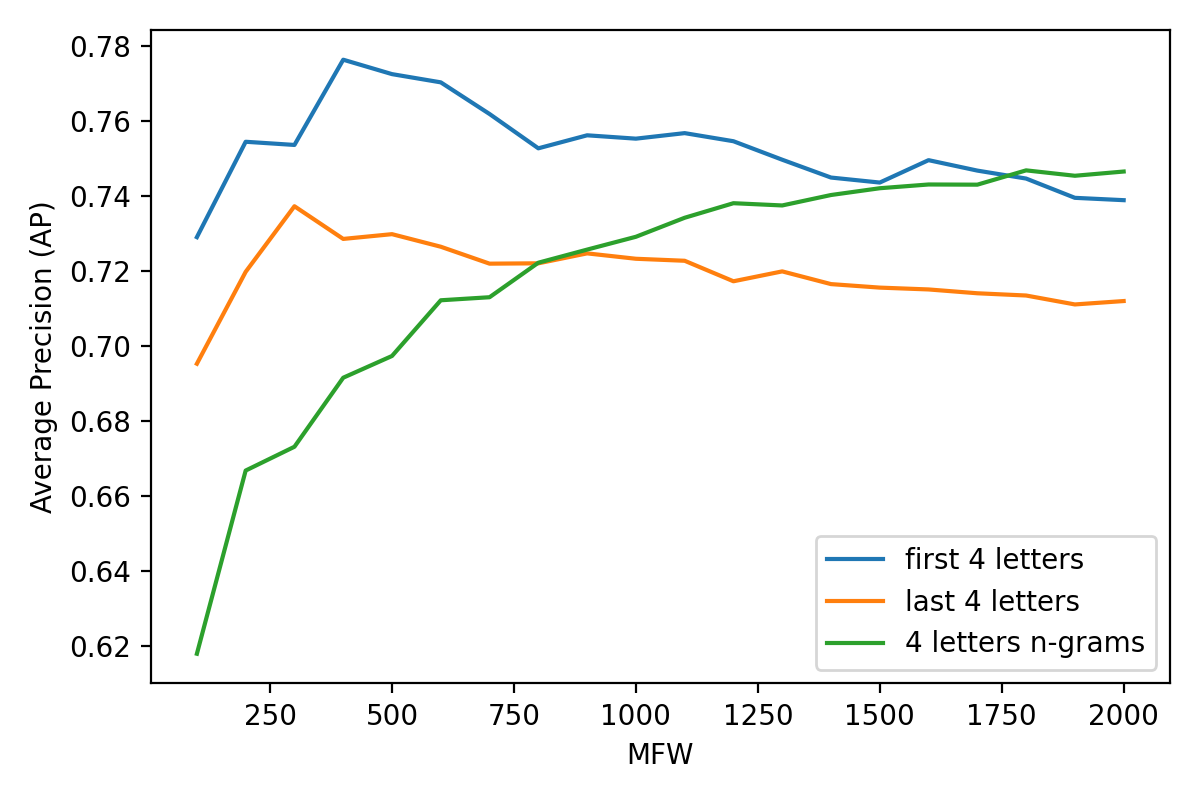
\includegraphics[width=\linewidth]{img/first_last_letters_ngrams.png}
  \caption{Average precision over the MFW in the rank list generated using the z-score normalized cosine distance.}
  \label{fig:first_last_letters_ngrams}
\end{figure}

\subsection{Clustering evaluation}

\begin{definition}[Correctness~\cite{bcubed}]
  Let L(e) and C(e) be the category and the cluster of an element e.
  The correctness has a value of one if the two elements are in the both in the same cluster and has the same category OR both in a different cluster and a different category. ($A \Longleftrightarrow B \equiv (A \land B) \lor (\neg A \land \neg B)$)
  \begin{gather*}
    Correctness(e, e') = \\
    \begin{cases}
      1, & if (L(e) = L(e')) \Longleftrightarrow (C(e) = C(e'))\\
      0, & otherwise
    \end{cases}
  \end{gather*}
\end{definition}

\begin{definition}[Precision $BCubed$~\cite{bcubed}]
  The average of correctness for all elements on the average of all element such that their cluster is the same.
  \begin{equation}
    BCubed_{precision} = \text{Avg}_{e}[\text{Avg}_{e' C(e)=C(e')}[Correctness(e, e')]]
  \end{equation}
\end{definition}

\begin{definition}[Recall $BCubed$~\cite{bcubed}]
  The average of correctness for all elements on the average of all element such that their category is the same.
  \begin{equation}
    BCubed_{recall} = \text{Avg}_{e}[\text{Avg}_{e' L(e)=L(e')}[Correctness(e, e')]]
  \end{equation}
\end{definition}

\begin{definition}[$BCubed F_1$ Score~\cite{bcubed}]
  The harmonic mean between the $BCubed_{precision}$ and $BCubed_{recall}$
  \begin{equation}
    BCubed_{F_1} =
    2 \cdot \frac{BCubed_{precision} \cdot BCubed_{recall}}
    {BCubed_{precision} + BCubed_{recall}}
  \end{equation}
\end{definition}


\subsubsection{Frequent errors}

This section, try to understand the errors in our system, in this case the false links (document pairs with different authors) highly ranked on different rank list.
The rank list quality is highly based on the feature vector created using the N-MFW, having a good understanding of this vector give good indications of the strength of the system.

To find reccurant errors in our system we use 5 different distance metrics on the relative frequency of the 500-MFW using the St-Jean dataset.
This generate 5 rank lists.
The average precision for these rank list is always greater than 0.7.
With this 5 rank lists only the top 10 false links are kept to be analyzed.
Frequent errors are link that appear often in this top 10.
Figures~\ref{fig:mfw_vector_error_0}~/~\ref{fig:mfw_vector_error_1} show two pairs (Zola 49 / Flaubert 63 and Maupassant 10 / Flaubert 52) that appear 4 time out of the 5 rank lists in the top 10 false links, thus frequent error.

\begin{figure}
  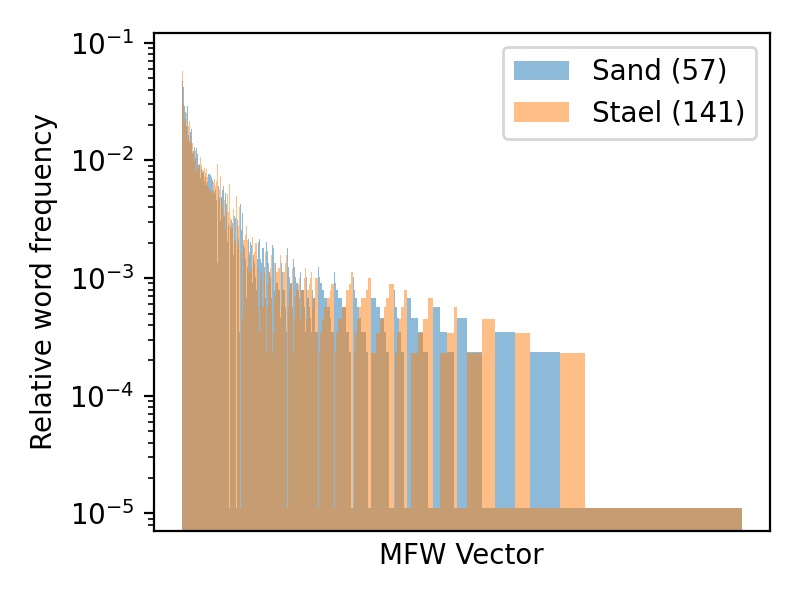
\includegraphics[width=\linewidth]{img/mfw_vector_error_0.png}
  \caption{First example of 500-MFW relative frequency vector for the two documents in a reccurant (4 rank lists out of 5) false link in the top 10 false links}
  \label{fig:mfw_vector_error_0}
\end{figure}
\begin{figure}
  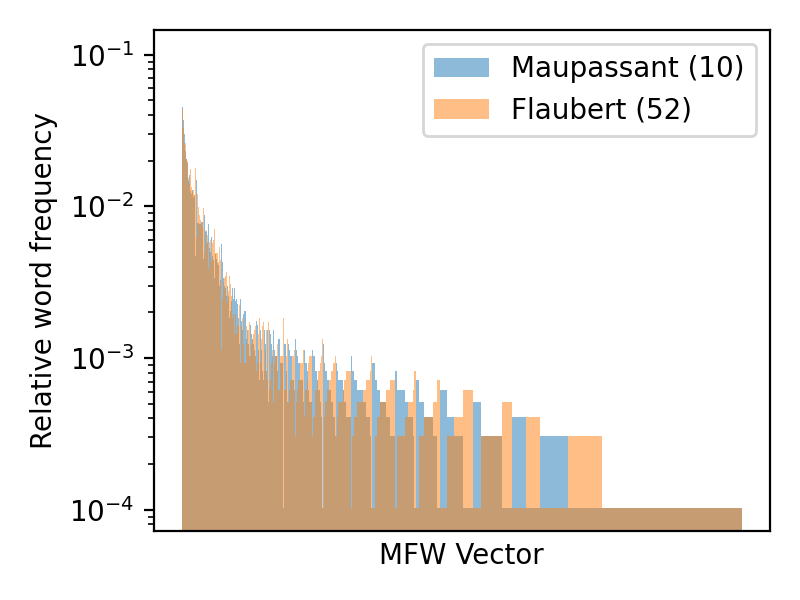
\includegraphics[width=\linewidth]{img/mfw_vector_error_1.png}
  \caption{Second example of 500-MFW relative frequency vector for the two documents in a reccurant (4 rank lists out of 5) false link in the top 10 false links}
  \label{fig:mfw_vector_error_1}
\end{figure}

To be able to understand more easily this vector, the values have been sorted by relative frequencies.
When a large propostion of the vectors overlap it indicates a high similarities between the vectors.
In this case most of the surface overlap so the distance function will give a low value, and rank this vector high in the list.
Both document style are close when their feature vector are closely related.
We can't clearly determinate that these texts are from different author using only this type of representation.
These two vectors pair can be vizually compared to the most similar link (ranked 1 using manhattan distance) in Figure~\ref{fig:mfw_vector_first_rl} (Stael 157 / Steal 183) or the HPrec-th (last continous correct pair from the top of the list) in Figure~\ref{fig:mfw_vector_first_last_rl} (Maupassant 10 / Maupassant 67), both of these links show a large propotion of overlapping surface.
A counter example would be the least similar link (ranked last using manhattan distance) which represent a negatively correlated document pair, Figure~\ref{fig:mfw_vector_last_rl} showcase this link.
As expected, most of this figure surface is non-overlapping.

\begin{figure}
  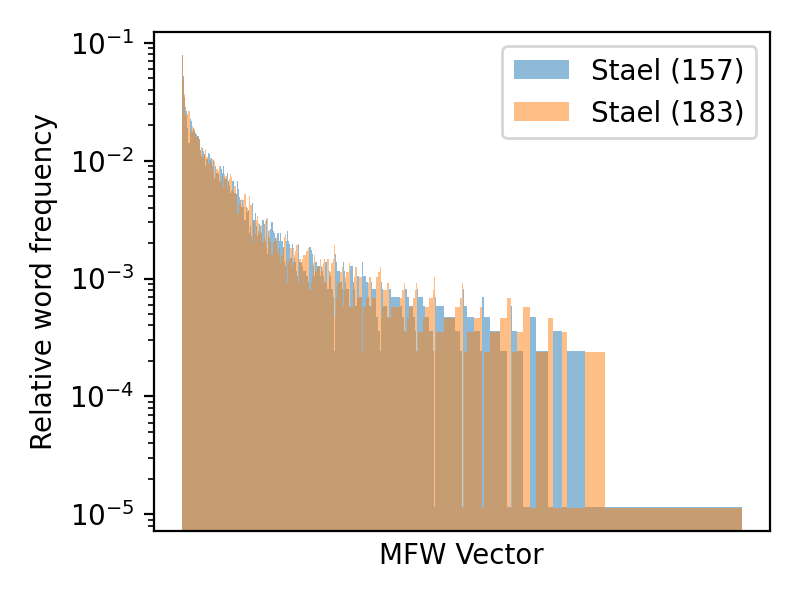
\includegraphics[width=\linewidth]{img/mfw_vector_first_rl.png}
  \caption{500-MFW relative frequency for the two documents ranked first in the rank list}
  \label{fig:mfw_vector_first_rl}
\end{figure}
\begin{figure}
  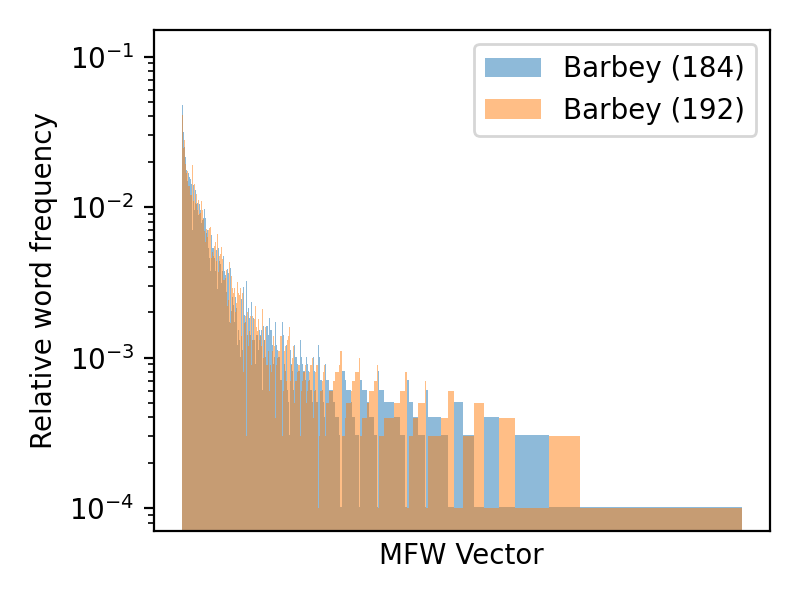
\includegraphics[width=\linewidth]{img/mfw_vector_first_last_rl.png}
  \caption{500-MFW relative frequency for the two documents ranked HPrec-th in the rank list}
  \label{fig:mfw_vector_first_last_rl}
\end{figure}
\begin{figure}
  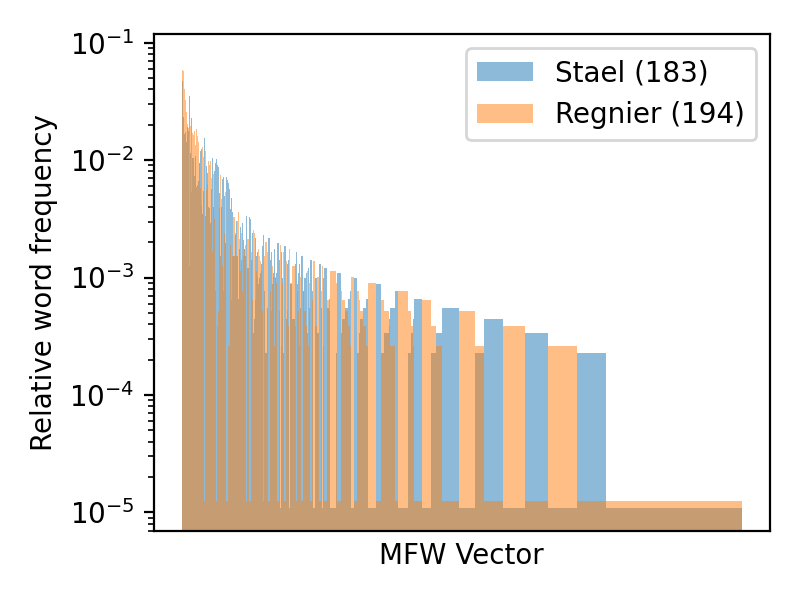
\includegraphics[width=\linewidth]{img/mfw_vector_last_rl.png}
  \caption{500-MFW relative frequency for the two documents ranked last in the ranked list}
  \label{fig:mfw_vector_last_rl}
\end{figure}

\subsubsection{Publication date differences analyis}

When dealing with false links ranked high in the rank list, as the previous experiment showed, some excerpt use similar words.
These shared words might be related to era the book was written.
The following experiment try to investigate on this.

First we must understand the publication date distribution of dataset. Figure~\ref{fig:dates_distribution} show this distribution.
Figure~\ref{fig:dates_differences_all} show the date difference distribution for each pairs of document, we can see that the average date difference in the dataset is 28.24 years with a standard deviation of 20.73 years.
Since this dataset contain multiple excerpt from the same book, we might consider only the links of differents authors (false links) Figure~\ref{fig:dates_differences_false} show such distribution.
As expected the mean increased to 29.04 years since there are less links with small date difference.
Same authors links (true links) are displayed in Figure~\ref{fig:dates_differences_r_true}, they confirm the previous statement that most of the same authors links have a low date difference with a mean at 5.11 years.

\begin{figure}
  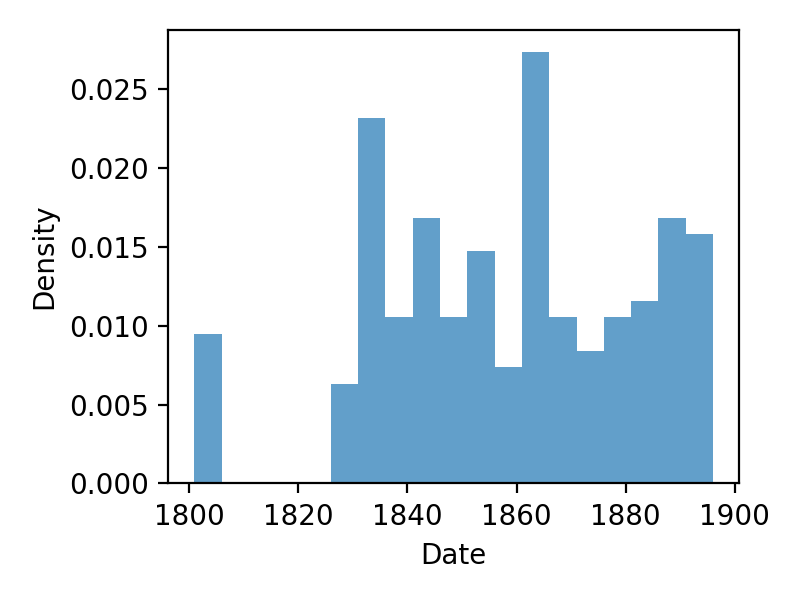
\includegraphics[width=\linewidth]{img/dates_distribution.png}
  \caption{Date distribution in the St-Jean dataset.}
  \label{fig:dates_distribution}
\end{figure}
\begin{figure}
  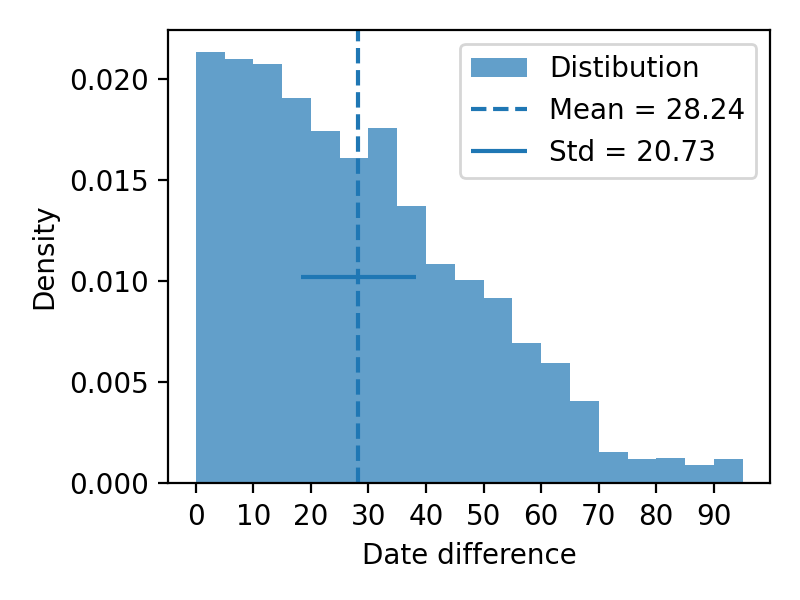
\includegraphics[width=\linewidth]{img/dates_differences_all.png}
  \caption{Pairwise date difference denstiy in St-Jean for all the excerpt.}
  \label{fig:dates_differences_all}
\end{figure}
\begin{figure}
  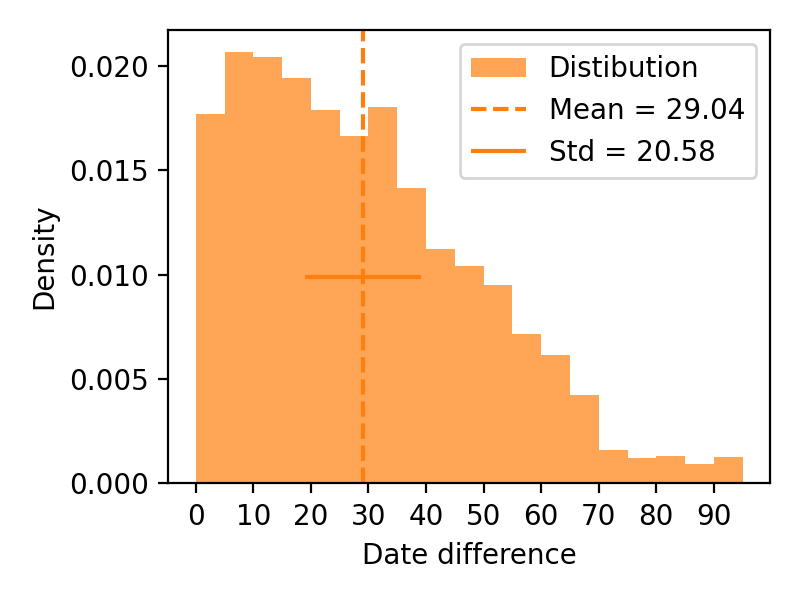
\includegraphics[width=\linewidth]{img/dates_differences_false.png}
  \caption{Pairwise date difference denstiy in St-Jean for all the excerpt with different authors (false links).}
  \label{fig:dates_differences_false}
\end{figure}
\begin{figure}
  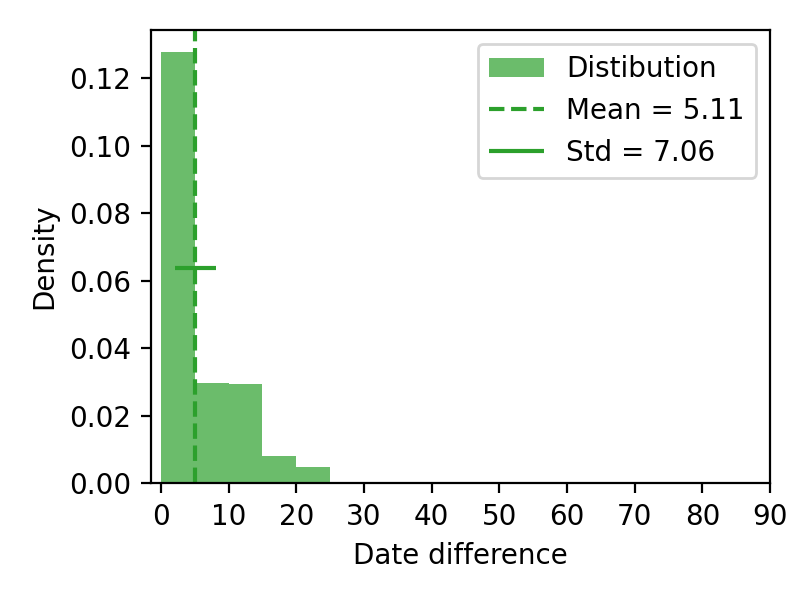
\includegraphics[width=\linewidth]{img/dates_differences_r_true.png}
  \caption{Pairwise date difference denstiy in St-Jean for all the excerpt with similar authors (true links) also correspond to the top-r true links.}
  \label{fig:dates_differences_r_true}
\end{figure}

Figure~\ref{fig:dates_differences_r_false} show the date difference density on the top-r false links (670 in case of St-Jean) on a rank list with 80\% average precision.
Two interesting informations can be extracted here.
First the mean is lower by 8.22 years (29.04 - 20.82) comparing to the false links distribution which clearly indicate a importance of publication date in the ranking of the documents.
Secondly we can obseve a drop at 35 years of date difference, which indicate that links in the interval $\left[0-35\right]$ are harder to discriminate than links outside this interval.
This 35 years interval can be related to the generation factor, the age of woman giving birth is around 25-34 in France \cite{generations}.
Each new generation use its own vocabulary and can be harder to discriminate author of text beloning to the same generation, in the other hand having differant vocabulary can indicate a differant time periode and is often use to detect document forgery \cite{savoy_stylo}.

\begin{figure}
  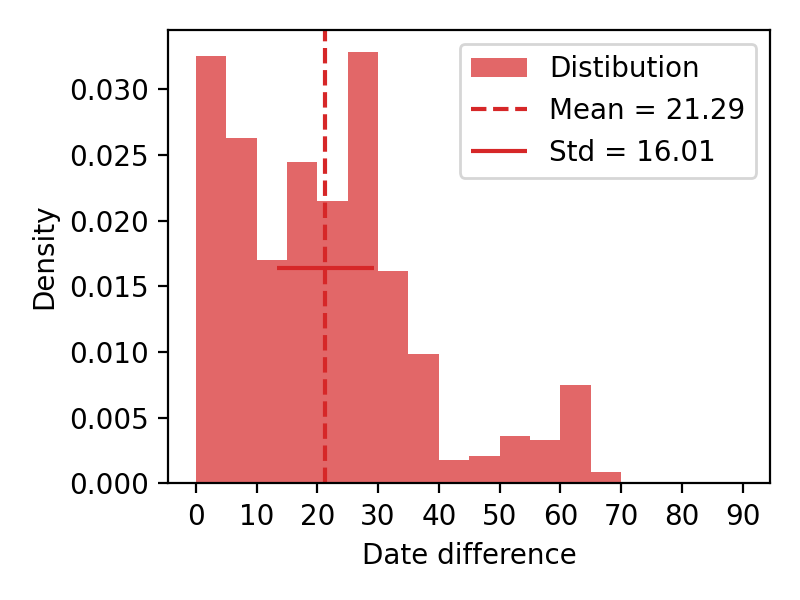
\includegraphics[width=\linewidth]{img/dates_differences_r_false.png}
  \caption{Pairwise date difference denstiy in St-Jean for top-r false links using a rank list with 80\% average precision.}
  \label{fig:dates_differences_r_false}
\end{figure}


\subsubsection{Rank lists fusion evaluation}

\begin{table}[h]
  \caption{\textbf{S-curve}/Equal/Linear,  * : Binomial test p-value < 5\%}
  \centering
  \label{}
  \begin{tabular}{l c c c}
    \toprule
    Metric & St-Jean & Brunet & Oxquarry \\ \midrule
    AP     & \textbf{*84/0/0} & \textbf{*67/0/17} & \textbf{*77/0/7} \\
    RPrec  & \textbf{*74/6/4} & \textbf{*31/38/15} & \textbf{*58/13/13} \\
    HPrec  & \textbf{*66/3/15} & \textbf{*20/54/10} & \textbf{40/17/27} \\
    \bottomrule
  \end{tabular}
\end{table}

\begin{table}[h]
  \caption{\textbf{S-curve}/Equal/Single max,  * : Binomial test p-value < 5\%}
  \centering
  \label{}
  \begin{tabular}{l c c c}
    \toprule
    Metric & St-Jean  & Brunet & Oxquarry \\ \midrule
    AP     & \textbf{*55/0/29} & 37/0/47 & 9/0/75* \\
    RPrec  & \textbf{*61/2/21} & \textbf{*52/15/17} & 1/2/81* \\
    HPrec  & \textbf{47/1/36} & 0/0/84* & 14/1/69* \\
    \bottomrule
  \end{tabular}
\end{table}

\begin{table}[h]
  \caption{\textbf{Linear}/Equal/Single max,  * : Binomial test p-value < 5\%}
  \centering
  \label{}
  \begin{tabular}{l c c c}
    \toprule
    Metric& St-Jean  & Brunet & Oxquarry \\ \midrule
    AP    & \textbf{50/0/34} & 26/0/58* & 4/0/80* \\
    RPrec & \textbf{*52/2/30} & \textbf{*50/14/20} & 3/1/80* \\
    HPrec & \textbf{44/0/40} & 0/0/84* & 14/0/70* \\
    \bottomrule
  \end{tabular}
\end{table}

\begin{figure}
  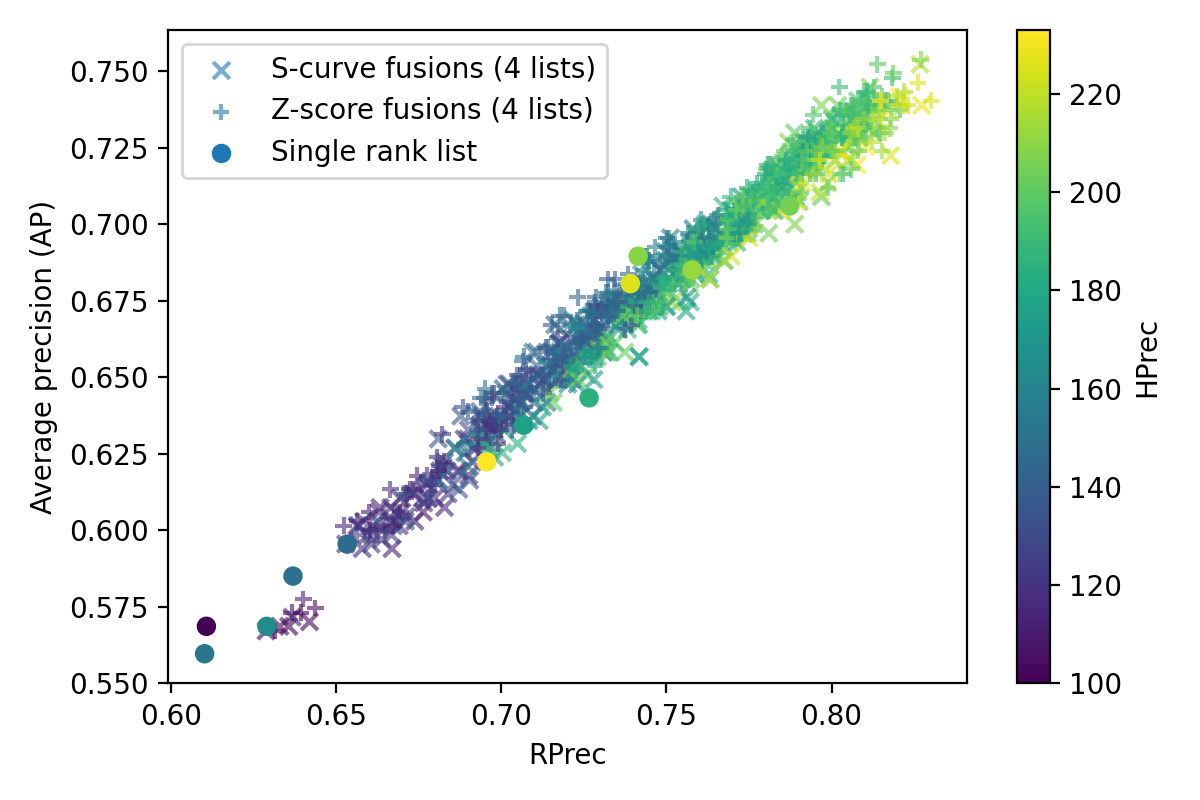
\includegraphics[width=\linewidth]{img/fusion_st_jean.png}
  \caption{}
  \label{fig:fusion_st_jean}
\end{figure}
\begin{figure}
  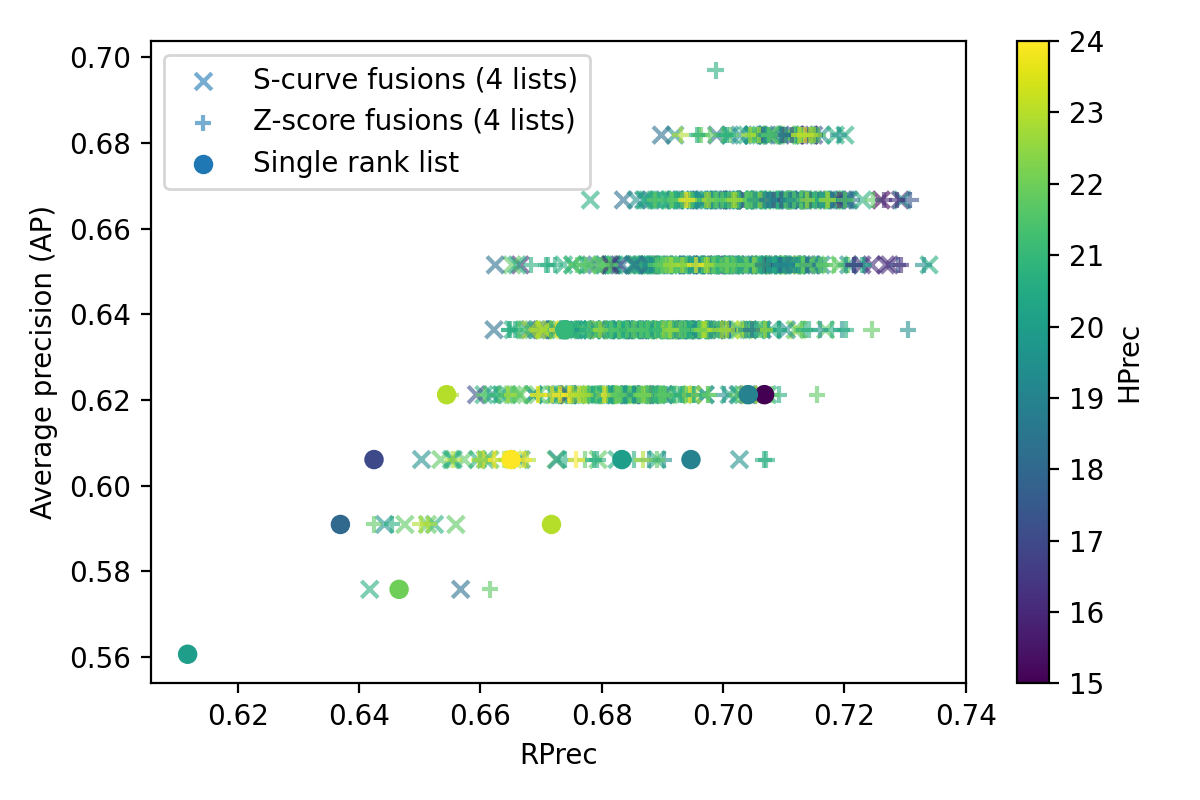
\includegraphics[width=\linewidth]{img/fusion_brunet.png}
  \caption{}
  \label{fig:fusion_brunet}
\end{figure}
\begin{figure}
  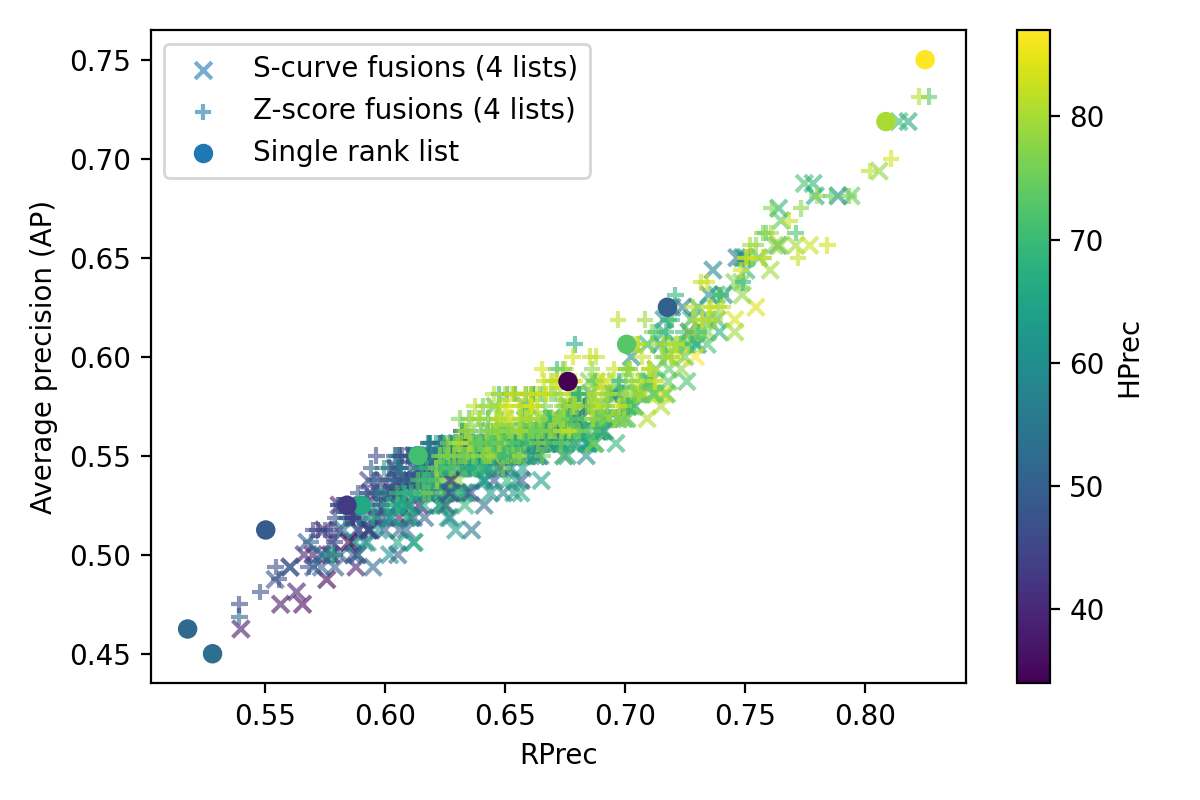
\includegraphics[width=\linewidth]{img/fusion_oxquarry.png}
  \caption{}
  \label{fig:fusion_oxquarry}
\end{figure}
